\documentclass[10pt,compress,t,notes=noshow, xcolor=table]{beamer}

% graphicx and color are loaded via lmu-lecture.sty
% maxwidth is the original width if it is less than linewidth
% otherwise use linewidth (to make sure the graphics do not exceed the margin)
% TODO: Remove once cleared to be superfluous
% \makeatletter
% \def\maxwidth{ %
%   \ifdim\Gin@nat@width>\linewidth
%     \linewidth
%   \else
%     \Gin@nat@width
%   \fi
% }
% \makeatother

% ---------------------------------%
% latex-math dependencies, do not remove:
% - mathtools
% - bm
% - siunitx
% - dsfont
% - xspace
% ---------------------------------%

%--------------------------------------------------------%
%       Language, encoding, typography
%--------------------------------------------------------%

\usepackage[english]{babel}
\usepackage[utf8]{inputenc} % Enables inputting UTF-8 symbols
% Standard AMS suite (loaded via lmu-lecture.sty)

% Font for double-stroke / blackboard letters for sets of numbers (N, R, ...)
% Distribution name is "doublestroke"
% According to https://mirror.physik.tu-berlin.de/pub/CTAN/fonts/doublestroke/dsdoc.pdf
% the "bbm" package does a similar thing and may be superfluous.
% Required for latex-math
\usepackage{dsfont}

% bbm – "Blackboard-style" cm fonts (https://www.ctan.org/pkg/bbm)
% Used to be in common.tex, loaded directly after this file
% Maybe superfluous given dsfont is loaded
% TODO: Check if really unused?
% \usepackage{bbm}

% bm – Access bold symbols in maths mode - https://ctan.org/pkg/bm
% Required for latex-math, preferred over \boldsymbol
% https://tex.stackexchange.com/questions/3238/bm-package-versus-boldsymbol
\usepackage{bm}

% pifont – Access to PostScript standard Symbol and Dingbats fonts
% Used for \newcommand{\xmark}{\ding{55}, which is never used
% aside from lecture_advml/attic/xx-automl/slides.Rnw
% \usepackage{pifont}

% Quotes (inline and display), provdes \enquote
% https://ctan.org/pkg/csquotes
\usepackage{csquotes}

% Adds arg to enumerate env, technically superseded by enumitem according
% to https://ctan.org/pkg/enumerate
% Replace with https://ctan.org/pkg/enumitem ?
% Even better: enumitem is not really compatible with beamer and breaks all sorts of things
% particularly the enumerate environment. The enumerate package also just isn't required
% from what I can tell so... don't re-add it I guess?
% \usepackage{enumerate}

% Line spacing - provides \singlespacing \doublespacing \onehalfspacing
% https://ctan.org/pkg/setspace
% \usepackage{setspace}

% mathtools – Mathematical tools to use with amsmath
% https://ctan.org/pkg/mathtools?lang=en
% latex-math dependency according to latex-math repo
\usepackage{mathtools}

% Maybe not great to use this https://tex.stackexchange.com/a/197/19093
% Use align instead -- TODO: Global search & replace to check, eqnarray is used a lot
% $ rg -f -u "\begin{eqnarray" -l | grep -v attic | awk -F '/' '{print $1}' | sort | uniq -c
%   13 lecture_advml
%   14 lecture_i2ml
%    2 lecture_iml
%   27 lecture_optimization
%   45 lecture_sl
\usepackage{eqnarray}
% For shaded regions / boxes
% Used sometimes in optim
% https://www.ctan.org/pkg/framed
\usepackage{framed}

%--------------------------------------------------------%
%       Cite button (version 2024-05)
%--------------------------------------------------------%

% Superseded by style/ref-buttons.sty, kept just in case these don't work out somehow.

% Note this requires biber to be in $PATH when running,
% telltale error in log would be e.g. Package biblatex Info: ... file 'authoryear.dbx' not found
% aside from obvious "biber: command not found" or similar.
% Tried moving this to lmu-lecture.sty but had issues I didn't quite understood,
% so it's here for now.

\usepackage{hyperref}

% Only try adding a references file if it exists, otherwise
% this would compile error when references.bib is not found
% NOTE: Bibliography packages (usebib, biblatex) are now loaded by ref-buttons.sty when needed
% This keeps all bibliography-related setup in one place

% Legacy \citelink command removed - superseded by ref-buttons.sty

%--------------------------------------------------------%
%       Displaying code and algorithms
%--------------------------------------------------------%

% Reimplements verbatim environments: https://ctan.org/pkg/verbatim
% verbatim used sed at least once in
% supervised-classification/slides-classification-tasks.tex
% Removed since code should not be put on slides anyway
% \usepackage{verbatim}

% Both used together for algorithm typesetting, see also overleaf: https://www.overleaf.com/learn/latex/Algorithms
% algorithmic env is also used, but part of the bundle:
%   "algpseudocode is part of the algorithmicx bundle, it gives you an improved version of algorithmic besides providing some other features"
% According to https://tex.stackexchange.com/questions/229355/algorithm-algorithmic-algorithmicx-algorithm2e-algpseudocode-confused
\usepackage{algorithm}
\usepackage{algpseudocode}

%--------------------------------------------------------%
%       Tables
%--------------------------------------------------------%

% multi-row table cells: https://www.namsu.de/Extra/pakete/Multirow.html
% Provides \multirow
% Used e.g. in evaluation/slides-evaluation-measures-classification.tex
\usepackage{multirow}

% colortbl: https://ctan.org/pkg/colortbl
% "The package allows rows and columns to be coloured, and even individual cells." well.
% Provides \columncolor and \rowcolor
% \rowcolor is used multiple times, e.g. in knn/slides-knn.tex
\usepackage{colortbl}

% long/multi-page tables: https://texdoc.org/serve/longtable.pdf/0
% Not used in slides
% \usepackage{longtable}

% pretty table env: https://ctan.org/pkg/booktabs
% Is used
% Defines \toprule
\usepackage{booktabs}

%--------------------------------------------------------%
%       Figures: Creating, placing, verbing
%--------------------------------------------------------%

% wrapfig - Wrapping text around figures https://de.overleaf.com/learn/latex/Wrapping_text_around_figures
% Provides wrapfigure environment -used in lecture_optimization
\usepackage{wrapfig}

% Sub figures in figures and tables
% https://ctan.org/pkg/subfig -- supersedes subfigure package
% Provides \subfigure
% \subfigure not used in slides but slides-tuning-practical.pdf errors without this pkg, error due to \captionsetup undefined
\usepackage{subfig}

% Actually it's pronounced PGF https://en.wikibooks.org/wiki/LaTeX/PGF/TikZ
\usepackage{tikz}

% No idea what/why these settings are what they are but I assume they're there on purpose
\usetikzlibrary{shapes,arrows,automata,positioning,calc,chains,trees, shadows}
\tikzset{
  %Define standard arrow tip
  >=stealth',
  %Define style for boxes
  punkt/.style={
    rectangle,
    rounded corners,
    draw=black, very thick,
    text width=6.5em,
    minimum height=2em,
    text centered},
  % Define arrow style
  pil/.style={
    ->,
    thick,
    shorten <=2pt,
    shorten >=2pt,}
}

%--------------------------------------------------------%
%       Beamer setup and custom macros & environments
%--------------------------------------------------------%

% Main sty file for beamer setup (layout, style, lecture page numbering, etc.)
% For long-term maintenance, this may me refactored into a more modular set of .sty files
\usepackage{../../style/lmu-lecture}
% Custom itemize wrappers, itemizeS, itemizeL, etc
\usepackage{../../style/customitemize}
% Custom framei environment, uses custom itemize!
\usepackage{../../style/framei}
% Custom frame2 environment, allows specifying font size for all content
\usepackage{../../style/frame2}
% Column layout macros
\usepackage{../../style/splitV}
% \image and derivatives
\usepackage{../../style/image}
% New generation of reference button macros
\usepackage{../../style/ref-buttons}

% Used regularly
\let\code=\texttt

% Not sure what/why this does
\setkeys{Gin}{width=0.9\textwidth}

% -- knitr leftovers --
% These may be used by knitr/R Markdown workflows in other lectures
\makeatletter
\def\maxwidth{ %
  \ifdim\Gin@nat@width>\linewidth
    \linewidth
  \else
    \Gin@nat@width
  \fi
}
\makeatother

% Define colors for syntax highlighting (may be used by knitr)
\definecolor{fgcolor}{rgb}{0.345, 0.345, 0.345}
\definecolor{shadecolor}{rgb}{.97, .97, .97}

% knitr code output environment
\newenvironment{knitrout}{}{}


% Can't find a reason why common.tex is not just part of this file?
% This file is included in slides and exercises

% Rarely used fontstyle for R packages, used only in 
% - forests/slides-forests-benchmark.tex
% - exercises/single-exercises/methods_l_1.Rnw
% - slides/cart/attic/slides_extra_trees.Rnw
\newcommand{\pkg}[1]{{\fontseries{b}\selectfont #1}}

% Spacing helpers, used often (mostly in exercises for \dlz)
\newcommand{\lz}{\vspace{0.5cm}} % vertical space (used often in slides)
\newcommand{\dlz}{\vspace{1cm}}  % double vertical space (used often in exercises, never in slides)
\newcommand{\oneliner}[1] % Oneliner for important statements, used e.g. in iml, algods
{\begin{block}{}\begin{center}\begin{Large}#1\end{Large}\end{center}\end{block}}

% Don't know if this is used or needed, remove?
% textcolor that works in mathmode
% https://tex.stackexchange.com/a/261480
% Used e.g. in forests/slides-forests-bagging.tex
% [...] \textcolor{blue}{\tfrac{1}{M}\sum^M_{m} [...]
% \makeatletter
% \renewcommand*{\@textcolor}[3]{%
%   \protect\leavevmode
%   \begingroup
%     \color#1{#2}#3%
%   \endgroup
% }
% \makeatother


% Defines macros and environments
% This file is included in slides and exercises

% Rarely used fontstyle for R packages, used only in 
% - forests/slides-forests-benchmark.tex
% - exercises/single-exercises/methods_l_1.Rnw
% - slides/cart/attic/slides_extra_trees.Rnw
\newcommand{\pkg}[1]{{\fontseries{b}\selectfont #1}}

% Spacing helpers, used often (mostly in exercises for \dlz)
\newcommand{\lz}{\vspace{0.5cm}} % vertical space (used often in slides)
\newcommand{\dlz}{\vspace{1cm}}  % double vertical space (used often in exercises, never in slides)
\newcommand{\oneliner}[1] % Oneliner for important statements, used e.g. in iml, algods
{\begin{block}{}\begin{center}\begin{Large}#1\end{Large}\end{center}\end{block}}

% Don't know if this is used or needed, remove?
% textcolor that works in mathmode
% https://tex.stackexchange.com/a/261480
% Used e.g. in forests/slides-forests-bagging.tex
% [...] \textcolor{blue}{\tfrac{1}{M}\sum^M_{m} [...]
% \makeatletter
% \renewcommand*{\@textcolor}[3]{%
%   \protect\leavevmode
%   \begingroup
%     \color#1{#2}#3%
%   \endgroup
% }
% \makeatother


\title{Interpretable Machine Learning}
% \author{LMU}
%\institute{\href{https://compstat-lmu.github.io/lecture_iml/}{compstat-lmu.github.io/lecture\_iml}}
\date{}

\begin{document}

\titlemeta{
Introduction to Feature Effects
}{
Interpretable Machine Learning
}{
figure/feature-effect
}{

\item Global Feature Effects
\item Local Feature Effects
%\item Understand how to interpret ICE curves and PD plots

}


% \begin{frame}{Feature Effects - Global View}

% %Here,

% %Here, the marginal effect of a feature $x_j$ does not vary across observations and is quantified by its associated coefficient $\hat\theta_j$. %, which explains how a feature affects the model prediction.

% %The $\hat\theta$-coefficients are constant across different observations.
% %It is sufficient to consider a feature's $\hat\theta$ coefficient as marginal effect as it provides an understanding how a feature affects the model prediction. % on average.

% %\lz
% % \textbf{Example}: %Visualizing the marginal effect of a LM (left) and a GAM (right) with a single feature (temperature) to predict the number of bike rentals.
% % Feature effect of LM (left) visualizes relationship of a single feature (here: temperature) on prediction (here: number of bike rentals) while ignoring all other features.
% % GAM (right) replaces linear terms $x_j\hat\theta_j$ of LM by non-linear functions $f_j(x_j)$ estimated via splines.
% %Marginal effects of a LM with features temperature (\texttt{temp}) and \texttt{season} to predict the number of bike rentals (\texttt{cnt}).

% \centering
% %\includegraphics[width=0.75\textwidth, trim=0cm 0.56cm 0cm 0.08cm, clip]{figure_man/lm_main_effects}

% \includegraphics[width=0.375\textwidth, trim=0cm 0.1cm 10.4cm 0cm, clip]{figure/lm_main_effects}\phantom{\includegraphics[width=0.375\textwidth, trim=10cm 0.1cm 0.4cm 0cm, clip]{figure/lm_main_effects}}

% LM without interaction: $\hat\theta_j$ is linear effect of feature $x_j$ (applies globally to all observations):
% %the prediction of any observation $\xi$ is %can be expressed by %explained by its marginal feature effects
% %prediction of an observation $\xi$ can be explained by the individual main effects, e.g.:
% $$\fh(\xv) = \hat\theta_0 + x_1\hat\theta_1$$ % + \dots + x_p\hat\theta_p.$$

% %\phantom{\includegraphics[width=0.375\textwidth, trim=0cm 0.1cm 10.4cm 0cm, clip]{figure/lm_main_effects}}\includegraphics[width=0.375\textwidth, trim=10cm 0.1cm 0.4cm 0cm, clip]{figure/lm_main_effects}

% % \begin{tabular}{c@{}c}
% %  \includegraphics[width=0.4\textwidth,trim=0cm 0.1cm 10.4cm 0cm,clip]{figure/lm_main_effects}\pause% 
% % &\includegraphics[width=0.4\textwidth,trim=10cm 0.1cm 0.4cm 0cm 0,clip]{figure/lm_main_effects}
% % \end{tabular}
% \end{frame}


\begin{frame}{Feature Effects - Global View}
%\includegraphics[width=0.375\textwidth, trim=0cm 0.1cm 10.4cm 0cm, clip]{figure/lm_main_effects}\phantom{\includegraphics[width=0.375\textwidth, trim=10cm 0.1cm 0.4cm 0cm, clip]{figure/lm_main_effects}}

\begin{columns}[T, totalwidth=\textwidth]
\begin{column}{0.49\linewidth}
\includegraphics[width=0.85\textwidth, trim=0cm 0.1cm 10.4cm 0cm, clip]{figure/lm_main_effects}

\bigskip
LM without interaction: $\hat\theta_j$ is linear effect of feature $x_j$ (applies globally to all obs.):
\begin{itemize}
    \item Model equation: $\fh(\xv) = \hat\theta_0 + x_1\hat\theta_1$
    \item Scalar $\hat\theta_1$ describes global effect
\end{itemize}
%$$% + \dots + x_p\hat\theta_p.$$
\end{column}\pause
\begin{column}{0.49\linewidth}
\invisible<1>{\includegraphics[width=0.85\textwidth, trim=10cm 0.1cm 0.4cm 0cm, clip]{figure/lm_main_effects}}

\bigskip
GAM without interaction: $\fh_j(x_j)$ is non-lin. effect of feature $x_j$  (applies globally):
\begin{itemize}
    \item Model equation: $\fh(\xv) = \hat\theta_0 + \fh_1(x_1)$
    \item Curve $\fh_1$ describes global effect
\end{itemize}
%$$% + \dots + \hat{h}_p(x_p).$$
\end{column}
\end{columns}

\end{frame}


\begin{frame}{Feature Effects - Localized View}

\centerline{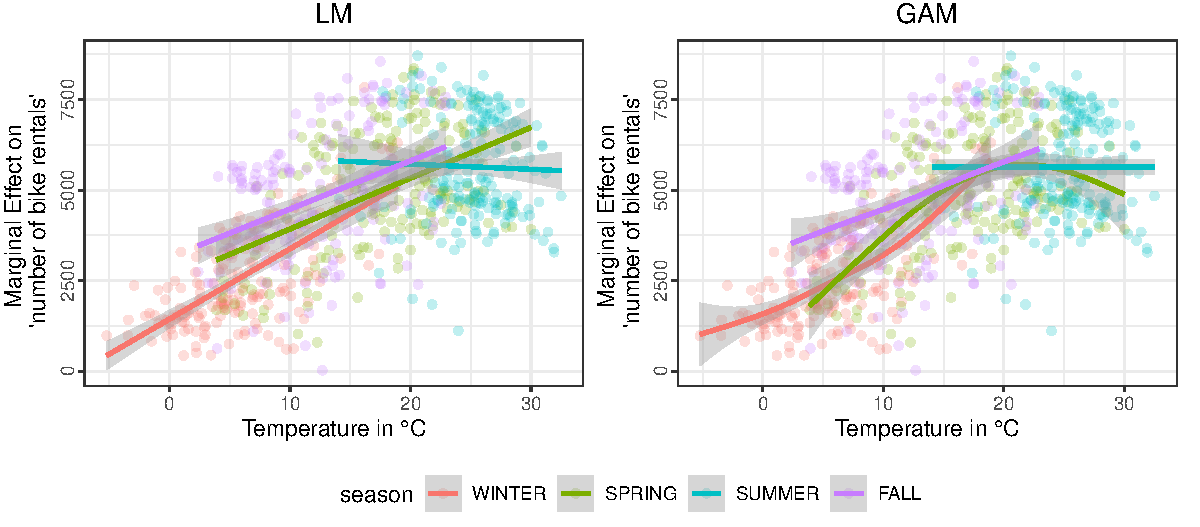
\includegraphics[width=0.8\textwidth, trim=0cm 0.1cm 0cm 0cm, clip]{figure/lm_main_interactions}}

\begin{itemize}
    \item \textbf{Interactions:} Feature effect depends on other features and varies across obs. \\ 
    $\Rightarrow$ E.g., effect of \textbf{temperature} varies across \textbf{season}\\
    $\Rightarrow$ Multiple values / curves needed to describe effect
    \item ML models capture non-linear effects and high-order interactions \\
    $\Rightarrow$ Global view often misleading (single curve may fail to capture complexity)\\
    $\Rightarrow$ Need for local feature effect methods to estimate effects for individual obs.\\
    %Need for local feature effect methods, e.g., analyze effect for individual obs.\\
    $\Rightarrow$ Global view can be reconstructed by aggregating local effects
\end{itemize}

\end{frame}

%
% \begin{frame}{Feature Effects}
%
% %If the model contains interactions, the global effect is not enough as the
% %If the model contains interactions, there is a modifying effect for certain observations that changes the slope of the regression line (in case of LMs) or the shape of the partial effect curve (in case of GAMs).
% %(in case of LMs) or the shape of the partial effect curve (in case of GAMs).
% %If the model contains interactions, the slope of the regression line (in case of LMs) or the shape of the partial effect curve (in case of GAMs) will be different for certain observations.
% If the model contains interactions, the functional shape of the estimated feature effect will usually be different for certain observations.
% \lz
%
% \textbf{Example}: If we include the interaction \texttt{temp*season},
% %the marginal effect of \texttt{temp} will depend on \texttt{season}. That is,
% observations belonging to a certain category of \texttt{season} will have different marginal effects (slopes) for \texttt{temp}.
% %, which results in a different slope for the feature temp at each category of the feature season.
% %so that each category of season yields a different slope for temp.
%
% {\centering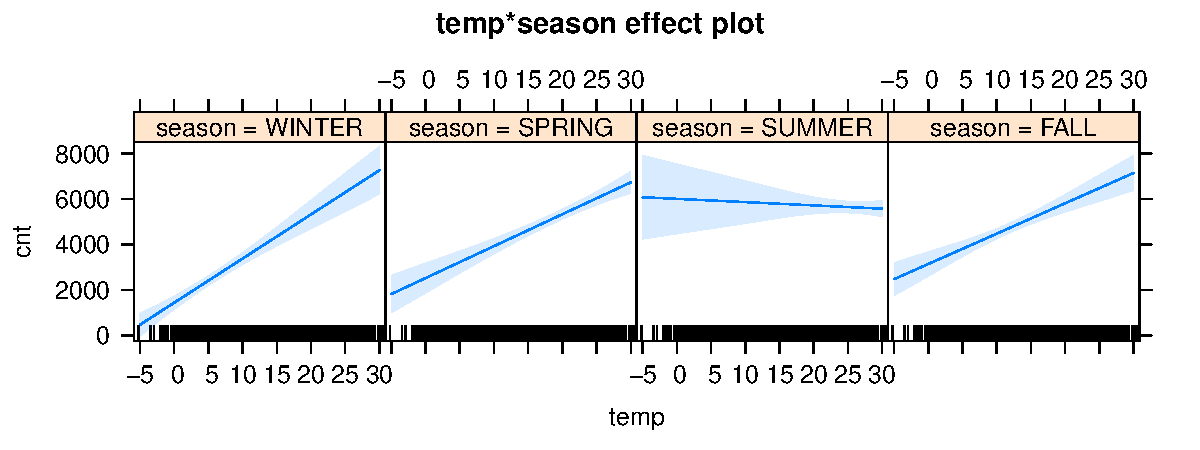
\includegraphics[width=0.9\textwidth, trim=0cm 0.1cm 0cm 0cm, clip]{figure_man/lm_interaction}}
%
% %\textbf{Note}: In case of interactions between two continuous features, we would obtain multiple regression lines with different slopes.
% %The marginal effect can then be visualized in a 2d effect plot or
%
% \end{frame}



\begin{frame}{Feature Effects}

\textbf{Feature effects} visualize or quantify how model predictions change as a single feature varies, while all other features are held fixed.
%marginal contribution of a feature of interest w.r.t. predictions %marginal contribution of a feature to the model \textbf{prediction}. % $\hat{y} = \fh(\xi[])$. effect (e.g., the average relationship) between a
\begin{itemize}
%\tightlist
\item Analogous to regression coefficients (LMs) or Splines (GAMs)
\item Different aggregation levels exist (simplification but information loss)
\item Methods: \visible<1-3>{ICE curves (local curves)}\visible<2-3>{, PD and ALE plots (global curves)}\visible<3>{, AME (global value)}
\end{itemize}

%\centerline{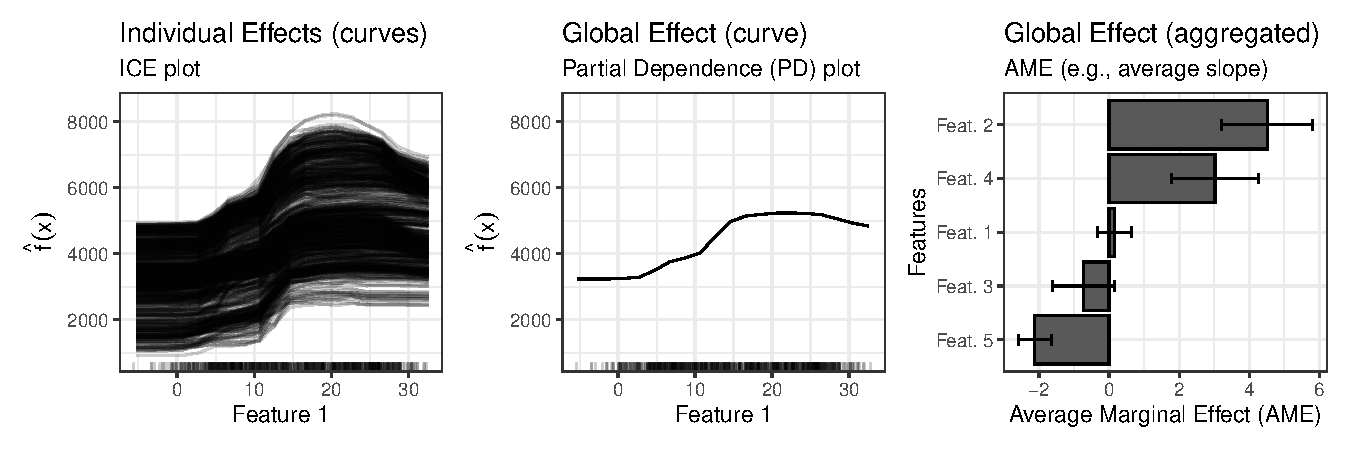
\includegraphics[width=\textwidth]{figure/feature-effect.pdf}}
\centerline{
\visible<1-3>{\adjincludegraphics[width=0.32\textwidth, trim={0 0 {.6667\width} 0}, clip]{figure/feature-effect.pdf}}
\visible<2-3>{\adjincludegraphics[width=0.32\textwidth, trim={{.33\width} 0 {.33\width} 0}, clip]{figure/feature-effect.pdf}}
\visible<3>{\adjincludegraphics[width=0.32\textwidth, trim={{.6667\width} 0 0 0}, clip]{figure/feature-effect.pdf}}
}

\smallskip
%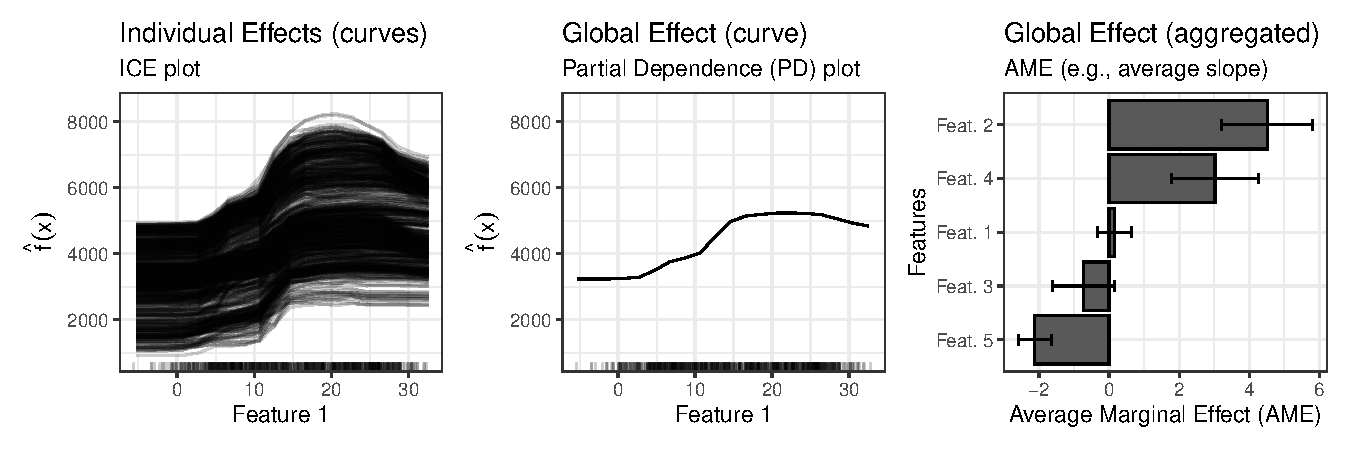
\includegraphics[width=0.33\textwidth, trim=7.4cm 0.1cm 7.4cm 0cm, clip]{figure/feature-effect.pdf}
%\invisible<1>{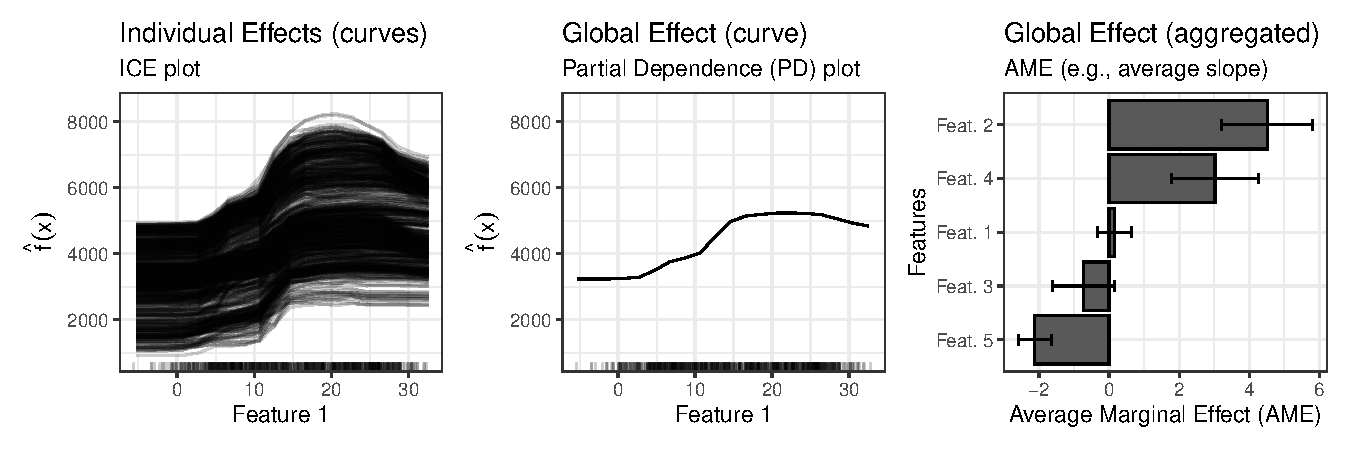
\includegraphics[width=0.33\textwidth, trim=14cm 0.1cm 0.4cm 0cm, clip]{figure/feature-effect.pdf}}

\small  \visible<1-3>{Individual (curves) \hspace{4px}}
\visible<2-3>{$\xrightarrow[\text{curves}]{\text{aggregate}}$ \hspace{4px} Global (single curve)}\visible<3>{\hspace{4px}
$\xrightarrow[\text{slopes}]{\text{aggregate}}$ \hspace{4px} Global (single value)}


\end{frame}


\endlecture
\end{document}
